\chapter{Experiments}

To investigate our research questions, we ran a series of experiments.
Recall the three research questions we wish to answer from Section \ref{sec:intro-problem-statement}, which can be summarized as: 1) How well does DARLInG perform overall, 2) what is the performance difference in using a one-hot encoding compared to a probability measure (PM) representation of the domain embedding, and 3) how does changing the signal-to-image transformation affect model performance?

In this chapter, we will first take a look at the preliminary experiments performed to verify that our model is adequate for the task at hand.
We will then discuss the experimental setup used to answer our research questions as well as the results of the experiments.

\section{Preliminary Experiments}\label{sec:experiments-preliminary}

We perform two preliminary experiments: running the VAE component only on a single-domain split of the dataset to ensure that the model is actually capable of classifying gestures and hyperparameter optimization to ensure that our experiments are being run with optimal hyperparameters.

\subsection{Single-Domain Experiments}

\begin{table}[t]
	\centering
	\begin{subtable}{0.3\textwidth}
		\centering
		\begin{tabular}{@{}lr@{}}
			\toprule
			Criteria       & Value \\ \midrule
			User           & 1     \\
			Room           & 1     \\
			Torso location & 1     \\
			Orientation    & 1     \\ \bottomrule
		\end{tabular}
		\caption{Single-domain split criteria.}
		\label{tab:single-domain-select}
	\end{subtable}
	\hfill
	\begin{subtable}{0.68\textwidth}
		\centering
		\begin{tabular}{@{}lrr@{}}
			\toprule
			Criteria       & Training Split      & Testing Split \\ \midrule
			User           & 3, 5, 10, 11, 12    & 1             \\
			Room           & 1                   & 1             \\
			Torso location & 1, 2, 3, 4, 5       & 1, 2, 3, 4, 5 \\
			Orientation    & 1                   & 1             \\ \bottomrule
		\end{tabular}
		\caption{Single user leave out criteria.}
		\label{tab:single-user-select}
	\end{subtable}
	\caption{Selection criteria for samples in our experiments with the Widar 3.0 dataset.}

\end{table}

\begin{table}[b]
	\centering
	\begin{tabular}{@{}lrrr@{}}
		\toprule
		Input modality     & Accuracy & Precision & F1-Score        \\ \midrule
		BVP                & 0.9222   & 0.9091    & \textbf{0.9655} \\
		CSI                & 0.9023   & 0.9091    & \textbf{0.9120} \\ \bottomrule
	\end{tabular}
	\caption{DARLInG's VAE component's performance on gesture prediction on a single-domain split of the Widar 3.0 dataset.}
	\label{tab:single-domain-performance}
\end{table}

To ensure that the model is performing adequately for the purposes of this experiment, we first chose to run the VAE component with no RL component on a single-domain split of the data.
This is done to ensure that the model can actually perform gesture classification in the first place, given no domain shifts.

In this experiment, we selected for only a single user in a single room in a single location with a single orientation, the details of which are seen in Table \ref{tab:single-domain-select}, with a 70-30 split for training-testing.
As input, we provide our model with both the BVP as well as the CSI, after being passed through our pipeline discussed in Section \ref{sec:methodology-signal-preprocessing} and the GAF transformation.

This resulted in the performance seen in Table \ref{tab:single-domain-performance}.
Our results here show that DARLInG is in fact capable of performing gesture classification and provides us the confidence to continue with our experiments.

\subsection{Hyperparameter Optimization}
\begin{table}
	\centering
	\resizebox{\textwidth}{!}{
	\begin{tabular}{@{}lccr@{}}
		\toprule
		Parameter                      & Possible values                        & Value distribution & Optimized value      \\ \midrule
		\multicolumn{4}{c}{RL Embedding Agent}                                                                              \\ \midrule
		Start Epoch                    & $[0, 50]$                              & Int Uniform        & $15$                 \\ \midrule
		\multicolumn{4}{c}{Encoder}                                                                                         \\ \midrule
		Activation Function            & \{Leaky ReLU, SeLU, ReLU\}             & Uniform            & Leaky ReLU           \\
		Dropout                        & $[0, 0.9]$                             & Uniform            & $0.18$               \\
		Initial Kernel Size            & $[3, 12]$                              & Int Uniform        & $7$                  \\
		Latent Variables               & $[10, 100]$                            & Int Uniform        & $60$                 \\
		Num Conv Blocks                & $[1, 10]$                              & Int Uniform        & $3$                  \\ \midrule
		\multicolumn{4}{c}{Multi-task Module}                                                                               \\ \midrule
		Decoder Activation Function    & \{Leaky ReLU, SeLU, ReLU\}             & Uniform            & Leaky ReLU           \\
		Decoder Dropout                & $[0, 0.9]$                             & Uniform            & $0.26$               \\
		Classifier Activation Function & \{Leaky ReLU, SeLU, ReLU\}             & Uniform            & SeLU                 \\
		Classifier Dropout             & $[0, 0.9]$                             & Uniform            & $0.28$               \\
		Classifier num layeres         & $[1, 10]$                              & Uniform            & $4$                  \\ \midrule
		\multicolumn{4}{c}{Optimizer}                                                                                       \\ \midrule
		$\alpha$                       & $[1 \times 10^{-10}, 1]$               & log uniform        & $8 \times 10^{-5}$   \\
		Learning rate                  & $[1 \times 10^{-6}, 1 \times 10^{-2}]$ & uniform            & $2.2 \times 10^{-4}$ \\
		Optimizer                      & \{SGD, Adam\}                          & Uniform            & Adam                 \\ \bottomrule
	\end{tabular}
	}
	\caption{Hyperparameter tuning results. Each section covers a different grouping of hyperparameters affecting a different component or module of DARLInG.}
	\label{tab:hpoptim-results}
\end{table}

To ensure that our experiments are being run with the optimal hyperparameters, we perform hyperparameter tuning using Weights and Biases and their sweep feature \cite{wandb}.
We setup our sweep to use Bayesian Optimization, the details of which are out of the scope of this thesis but can be found in the author's bachelors thesis \cite{satyawan2019semantic}.
We utilize hyperparameter tuning extensively, running a total of 817 runs with each run running for 50 epochs.
The results of the hyperparameter tuning can be seen in Table \ref{tab:hpoptim-results} and was used for all further experiments.

\section{Experimental Setup and Results}\label{sec:experiments-setup-results}
\begin{table}[]
	\centering
	\resizebox{\textwidth}{!}{
	\begin{tabular}{@{}lllrrrrrr@{}}
		\toprule
		\multicolumn{1}{c}{} & \multicolumn{1}{c}{} & \multicolumn{1}{c}{} & \multicolumn{2}{c}{Accuracy} & \multicolumn{2}{c}{Precision} & \multicolumn{2}{c}{F1-Score} \\
		Transform            & RL Agent             & Encoding             & Null head    & Embed head    & Null head     & Embed head    & Null head    & Embed head    \\ \midrule
		GAF                  & -                    & Known                & 0.410        & 0.427         & 0.446         & 0.446         & 0.402        & \textbf{0.439}         \\
		GAF                  & PPO                  & PM                   & 0.339        & 0.357         & 0.339         & 0.357         & 0.339        & \textbf{0.357}         \\
		GAF                  & PPO                  & One-hot              & 0.366        & 0.384         & 0.366         & 0.384         & 0.339        & \textbf{0.354}         \\
		GAF                  & DDPG                 & PM                   & 0.371        & 0.367         & 0.384         & 0.384         & 0.364        & \textbf{0.378}         \\
		GAF                  & DDPG                 & One-hot              & 0.429        & 0.438         & 0.420         & 0.402         & 0.429        & \textbf{0.438}         \\
		MTF                  & -                    & Known                & 0.374        & 0.365         & 0.304         & 0.295         & 0.304        & \textbf{0.295}         \\
		MTF                  & PPO                  & PM                   & 0.286        & 0.321         & 0.286         & 0.321         & 0.369        & \textbf{0.384}         \\
		MTF                  & PPO                  & One-hot              & 0.464        & 0.446         & 0.464         & 0.446         & 0.384        & \textbf{0.393}         \\
		MTF                  & DDPG                 & PM                   & 0.378        & 0.391         & 0.402         & 0.420         & 0.371        & \textbf{0.395}         \\
		MTF                  & DDPG                 & One-hot              & 0.420        & 0.491         & 0.420         & 0.491         & 0.376        & \textbf{0.438}         \\
		RP                   & -                    & Known                & 0.375        & 0.384         & 0.375         & 0.384         & 0.375        & \textbf{0.384}         \\
		RP                   & PPO                  & PM                   & 0.325        & 0.331         & 0.339         & 0.348         & 0.328        & \textbf{0.326}         \\
		RP                   & PPO                  & One-hot              & 0.330        & 0.332         & 0.304         & 0.348         & 0.331        & \textbf{0.332}         \\
		RP                   & DDPG                 & PM                   & 0.411        & 0.429         & 0.411         & 0.429         & 0.379        & \textbf{0.419}         \\
		RP                   & DDPG                 & One-hot              & 0.392        & 0.397         & 0.375         & 0.384         & 0.389        & \textbf{0.404}         \\ \bottomrule
	\end{tabular}
	}
	\caption{Final experimental results of the performance of DARLInG by type of RL agent, domain embedding encoding, and signal-to-image transformation. Each pair of columns represents the results of the null head and the results of the embed head in each of the metrics accuracy, precision, and F1-score. The final F1-Score of the evaluation is emphasized in bold type.}
	\label{tab:final-results}
\end{table}

\begin{figure}
	\centering
	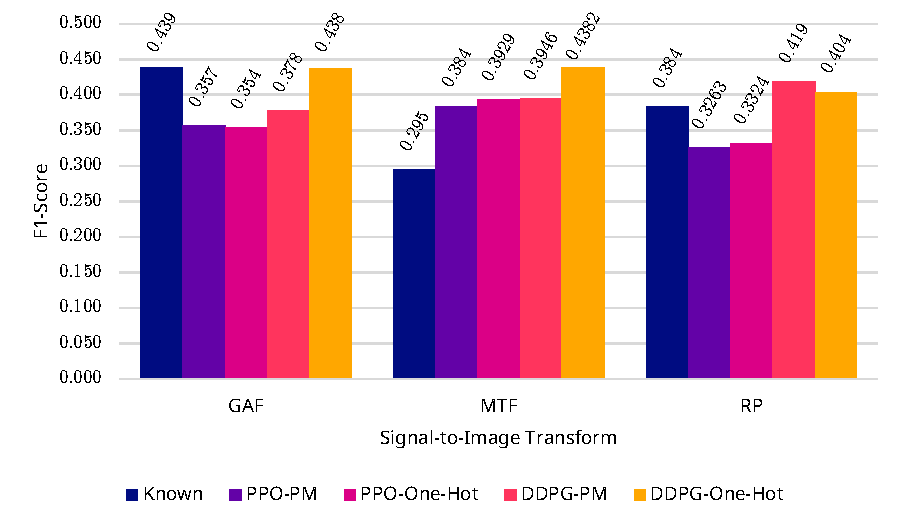
\includegraphics[width=6in]{figures/results_main}
	\caption{The summarized results of the experiments, showing F1-score grouped by the signal-to-image transform used. For each signal-to-image transform, the colors represent the RL algorithm and the encoding used.}
	\label{fig:results-main}
\end{figure}

\begin{figure}
	\centering
	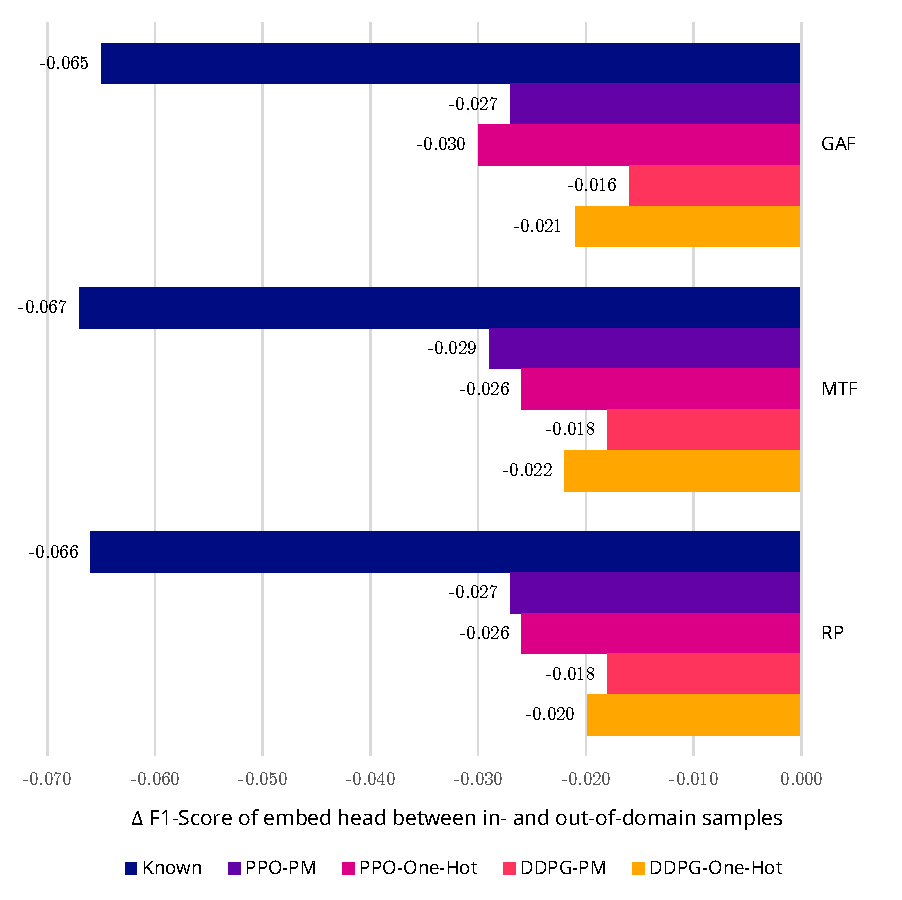
\includegraphics[width=6in]{figures/results_domains}
	\caption{The difference in performance of our models on in-domain vs. out-of-domain samples. The in-domain samples were taken from a held-out set of the training samples. The values are grouped by signal-to-image transform and the colors represent the RL algorithm and the encoding used. The shown values indicate the reduction in F1-score of our model on out-of-domain samples w.r.t. the in-domain samples with lower values indicating better performance on the in-domain samples.}
	\label{fig:results-domains}
\end{figure}
	
\begin{figure}
	\centering
	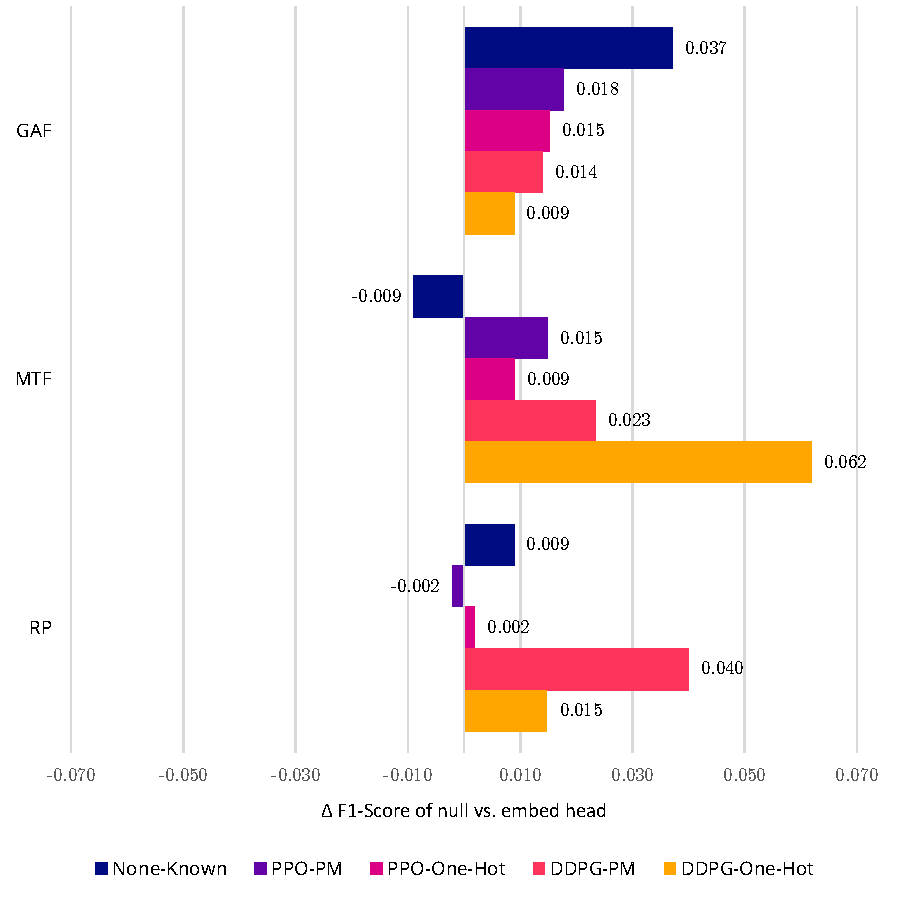
\includegraphics[width=6in]{figures/results_delta}
	\caption{This chart shows the performance delta between the null head and the embed head for each experiment. Higher positive values indicate that the embed head achieved a higher F1-score.}
	\label{fig:results-delta}
\end{figure}

\begin{figure}
	\centering
	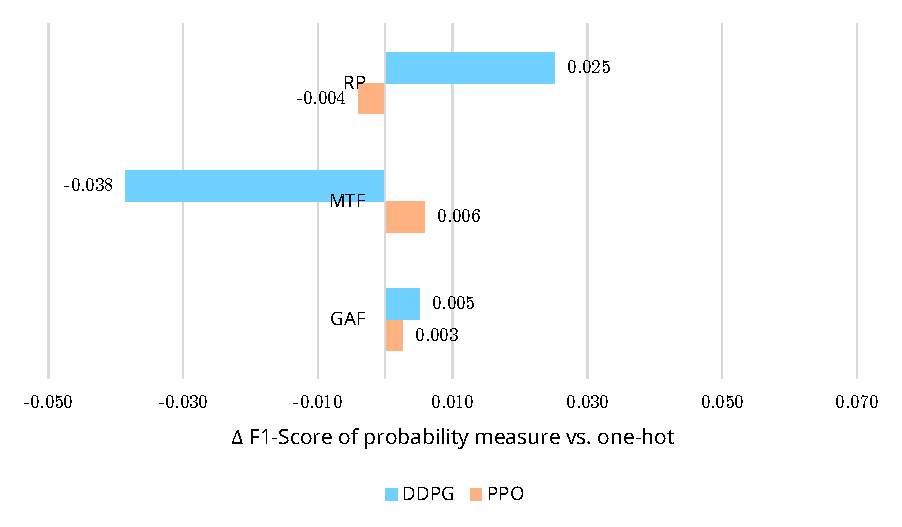
\includegraphics[width=6in]{figures/results_encoding}
	\caption{This chart shows the overall performance delta between using a probability measure and a one-hot encoding for the domain embedding. The values are grouped by signal-to-image transform and the colors represent the RL algorithm used. The scores used here have also been corrected for their respective algorithm's null head performance, i.e., uses the scores seen in Figure \ref{fig:results-delta} instead of in Table \ref{tab:final-results}. Higher positive values indicate the embed head achieved a higher F1-score when using the probability measure encoding as opposed to using a one-hot encoding.}
	\label{fig:results-encoding}
\end{figure}

To answer our research questions, we set up a series of experiments with single-user leave out validation.
The criteria used to choose which samples were used as training samples and which for testing are shown in Table \ref{tab:single-user-select} and resulted in a $\frac{2}{3}:\frac{1}{3}$ split of the data.
We additionally held $\frac{1}{10}$ of the training data as a hold-out split to test in- vs.\ out-of-domain performance of our model.
We chose these specific users due to them all being males of similar BMI, as seen in Figure 12 of \cite{zheng2019zero}.
Using this data, we set up experiments to answer our research questions from Section \ref{sec:intro-problem-statement}.
These experiments ran every combination of RL agent (PPO, DDPG, and known domain factors as a baseline), signal-to-image transform (GAF, MTF, and RP), and encoding method (probability-measure and one-hot) that we have previously chosen.

The results of our experimental runs can be seen in Table \ref{tab:final-results} and are visualized in Figure \ref{fig:results-main}.
This table, and every figure with experimental results, shows the final model performance on the test set.
In this table, we show the performance of DARLInG with two RL algorithms: PPO and DDPG, as well as when the embed head is provided the known domain factors.
For each embedding type, we encode the output as either a probability measure (PM) or as a one-hot encoded vector.
Finally, for each algorithm and encoding, we provide an input image of the CSI as transformed by GAF, MTF, and RP, details of which can be found in \ref{sec:background-signal-to-image}.

Another way to analyze our runs is to investigate the difference in performance of our model on in-domain vs. out-of-domain samples.
To do so, we ran our trained models on the held-out split of the training set.
The results can be seen in Figure \ref{fig:results-domains}.
These results indicate that in all cases, our model performs better on in-domain samples, as is expected.
The performance on out-of-domain samples are much worse on the known encoding, indicating that the known encoding of domain factors, while usable, is not great for out-of-domain samples.
Our results also support that DDPG performs best for out-of-domain samples.

The performance of the embed heads compared to their respective null heads can be seen in Figure \ref{fig:results-delta}, in which greater positive values indicate that the embed head is performing better than the null head.
We can see that with MTF and RP, DDPG out-performs PPO while PPO slightly outperforms DDPG with GAF.
Using known domain factors improves performance, but only with GAF and RP transforms while it has the decreases performance with MTF.
The largest increase in performance can be seen with MTF transforms and the DDPG RL algorithm with one-hot encoding.
Interestingly, PPO with RP seems to provide no actual benefit.

To answer our second research question, we compare the performance of a domain embedding encoded as a probability-measure and one using one-hot encoding, the results of which are seen in Figure \ref{fig:results-encoding}.
The results show that generally, the encoding method does not make a significant difference for PPO and only makes a difference for DDPG with MTF and RP transforms.
With the MTF transform, one-hot is the preferred encoding while in RP, the probability-measure is the prefered encoding.

Comparing all these results with the baseline of a known domain encoding, we see that although the known-domain encoding performs well with GAF and RP, and poorly on MTF, the known-domain encoding fails to provide an adequate representation of out-of-domain samples, as seen in Figure \ref{fig:results-domains}.
This may simply be to the discrete (i.e., categorical) encoding of the domain factors provided by the known domain encoding, instead of the more complex domain representations provided by the RL agents.
For example, although subject height is a continuous variable which can be properly encoded by a multi-dimensional one-hot encoding or a probability measure, a one-hot user encoding provides no further information about how height varies between two users.
This suggests that the RL agents provide a better encoding across domains, but fall short of hand-crafted domain labels with ground-truth information and no out-of-domain samples.

The results are generally unimpressive, though, with F1-scores significantly below both the baseline in \cite{zheng2019zero} and any of the state-of-the-art methods discussed in Chapter \ref{chapter:literature-review}.

\subsection{Extended Run}\label{subsec:experiments-longer}

\begin{table}[]
	\centering
	\begin{tabular}{@{}lr@{}}
		\toprule
		         & F1-Score \\ \midrule
		Standard & 0.438    \\
		Extended & 0.553    \\ \bottomrule
	\end{tabular}
	\caption{Extended training run results of the DDPG agent with MTF transform and one-hot encoding.}
\end{table}

As one final experiment, we ran our best performing configuration, i.e., DDPG with MTF transform and one-hot encoding, on the TU/e High-Performance Computing cluster with 100 model epochs and 50400 agent iterations per epoch.
The number of agent iterations were chosen as the closest full dataset iterations to 50000 steps, resulting in a total of 3528000 total agent steps as we set the agent training starting epoch $\zeta = 30$.
We double $\zeta$ to 30 as we also double the total number of epochs during training.
This is twice the training length of the VAE and 100$\times$ the training length for the agent relative to the other training runs.

We observe an increase in performance, with around a 12 percentage point increase in F1-score and the performance plateauing around epoch 75.
Although this is a welcome increase in performance, this is still below the baselines in \cite{zheng2019zero} and any of those discussed in Chapter \ref{chapter:literature-review}.
It does, however, rule out increasing training duration as a way to increase model performance.
